\section{Importance and difficulties}

Customer-provided requirements can be categorized into three primary types:
\begin{itemize}
    \item Functional requirements: These delineate the system's interactions with its environment, irrespective of implementation details. 
        They represent the core objectives that the software must achieve.
    \item Nonfunctional requirements: These encompass user-visible aspects of the system that aren't directly tied to functional behavior.
    \item Constraints: these restrictions are either set by the client or are inherent to the system's operational environment.
\end{itemize}
Nonfunctional requirements, often referred to as quality of service attributes, specify how functionality should be delivered to the end user. 
While they transcend specific application domains, their relevance and prioritization are influenced by the application's context.
\begin{figure}[H]
    \centering
    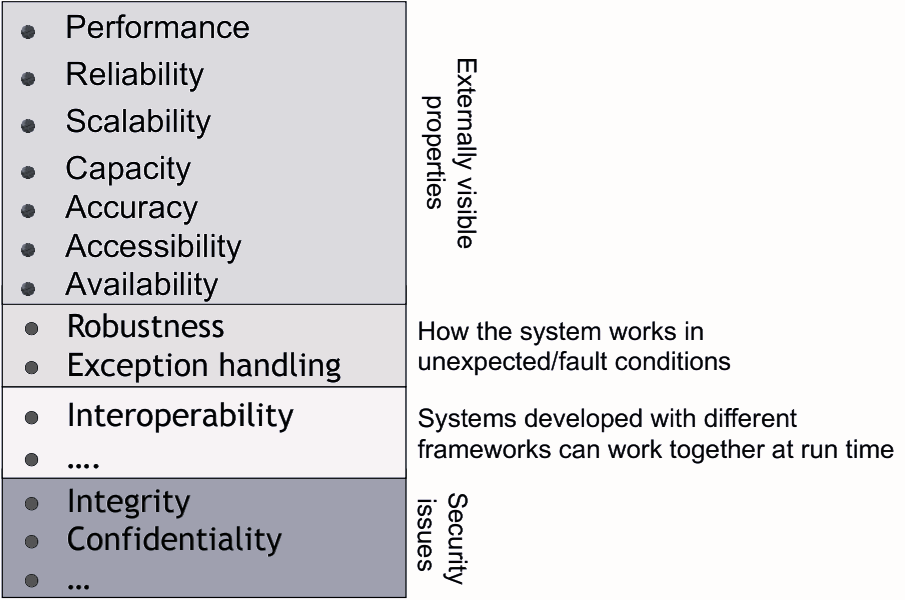
\includegraphics[width=0.35\linewidth]{images/QoS.png}
    \caption{Some relevant QoS characteristics}
\end{figure}